%% LyX 2.3.6.1 created this file.  For more info, see http://www.lyx.org/.
%% Do not edit unless you really know what you are doing.
\documentclass[12pt,preprint,3p]{elsarticle}
\usepackage[latin9]{inputenc}
\usepackage{float}
\usepackage{textcomp}
\usepackage{amstext}
\usepackage{amssymb}
\usepackage{graphicx}

\makeatletter

%%%%%%%%%%%%%%%%%%%%%%%%%%%%%% LyX specific LaTeX commands.
\DeclareTextSymbolDefault{\textquotedbl}{T1}
%% A simple dot to overcome graphicx limitations
\newcommand{\lyxdot}{.}


%%%%%%%%%%%%%%%%%%%%%%%%%%%%%% User specified LaTeX commands.
%%
%% Copyright 2007, 2008, 2009 Elsevier Ltd
%%
%% This file is part of the 'Elsarticle Bundle'.
%% ---------------------------------------------
%%
%% It may be distributed under the conditions of the LaTeX Project Public
%% License, either version 1.2 of this license or (at your option) any
%% later version.  The latest version of this license is in
%%    http://www.latex-project.org/lppl.txt
%% and version 1.2 or later is part of all distributions of LaTeX
%% version 1999/12/01 or later.
%%
%% The list of all files belonging to the 'Elsarticle Bundle' is
%% given in the file `manifest.txt'.
%%

%% Template article for Elsevier's document class `elsarticle'
%% with numbered style bibliographic references
%% SP 2008/03/01
%%
%%
%%
%% $Id: elsarticle-template-num.tex 4 2009-10-24 08:22:58Z rishi $
%%
%%


%% Use the option review to obtain double line spacing
%% \documentclass[preprint,review,12pt]{elsarticle}

%% Use the options 1p,twocolumn; 3p; 3p,twocolumn; 5p; or 5p,twocolumn
%% for a journal layout:
%% \documentclass[final,1p,times]{elsarticle}
%% \documentclass[final,1p,times,twocolumn]{elsarticle}
%% \documentclass[final,3p,times]{elsarticle}
%% \documentclass[final,3p,times,twocolumn]{elsarticle}
%% \documentclass[final,5p,times]{elsarticle}
%% \documentclass[final,5p,times,twocolumn]{elsarticle}

%% if you use PostScript figures in your article
%% use the graphics package for simple commands
%% \usepackage{graphics}
%% or use the graphicx package for more complicated commands
%% \usepackage{graphicx}
%% or use the epsfig package if you prefer to use the old commands
%% \usepackage{epsfig}

%% The amssymb package provides various useful mathematical symbols
%% The amsthm package provides extended theorem environments
%% \usepackage{amsthm}

%% The lineno packages adds line numbers. Start line numbering with
%% \begin{linenumbers}, end it with \end{linenumbers}. Or switch it on
%% for the whole article with \linenumbers after \end{frontmatter}.
%% \usepackage{lineno}

%% natbib.sty is loaded by default. However, natbib options can be
%% provided with \biboptions{...} command. Following options are
%% valid:

%%   round  -  round parentheses are used (default)
%%   square -  square brackets are used   [option]
%%   curly  -  curly braces are used      {option}
%%   angle  -  angle brackets are used    <option>
%%   semicolon  -  multiple citations separated by semi-colon
%%   colon  - same as semicolon, an earlier confusion
%%   comma  -  separated by comma
%%   numbers-  selects numerical citations
%%   super  -  numerical citations as superscripts
%%   sort   -  sorts multiple citations according to order in ref. list
%%   sort&compress   -  like sort, but also compresses numerical citations
%%   compress - compresses without sorting
%%
%% \biboptions{comma,round}

% \biboptions{}


%\journal{Nuclear Physics B}

\makeatother

\begin{document}

\part{Identification of fuel cells and electromagnetic reverberations chambers}

\section{Fuel cell}

\subsection{Fuel cell technology use}

Fuel cells belong to the group of galvanic elements, which, as electrochemical
energy converters, can convert the chemical energy of a fuel into
electrical energy. Since fuel cells can generate electricity directly
from chemical energy, they are much more efficient than internal combustion
engines \citep{Kurzweil2016}. The principle of the fuel cell was
discovered in 1838 by Christian Friedrich Sch�nbein and soon after,
Sir William Grove, along with Sch�nbein, recognized the reversal of
electrolysis and power generation. With the invention of the electrical
generator by Werner von Siemens, the invention known as the \textquotedbl gas
battery\textquotedbl{} fell into oblivion. It wasn't until the 1950s
that the idea was revived due to the need for compact and portable
power sources in space travel and the military. Global warming and
air pollution gave research into this technology decisive impetus
that continues to this day.

\subsection{Principle of operation}

A fuel cell consists of a cathode, anode coated with catalysts such
as platinum or nickel and a membrane Fig \ref{fig:Basic-structure-and}.

\begin{figure}[H]
\begin{centering}
\includegraphics[scale=0.3]{\string"images/reactionin fuel cellbearb.1\string".eps}
\par\end{centering}
\centering{}\caption{\label{fig:Basic-structure-and}Basic structure and functioning of
a fuel cell \citep{prezi.com}}
\end{figure}

The anode is supplied with hydrogen $\left[\textrm{\ensuremath{\mathsf{\textrm{H}}}}_{2}\right]$,
which oxidizes to protons $\left[2\mathsf{\textrm{H}}^{+}\right]$
on the catalyst layer, giving off electrons $\left[2\textrm{e}^{-}\right]$.
The proton exchange membran (PEM) is only permeable for ions, so only
the ions flow to the cathode via PEM. The electrons flow from the
anode to the cathode via an external circuit and form the electric
current. Both hydrogen protons and electrons migrate to the cathode,
where they react with the supplied oxygen $\left[\textrm{O}_{2}\right]$
to form water $\left[\textrm{H}_{2}\textrm{O}\right]$. Depending
on the operating point, a single cell delivers a certain voltage between
0.5 and 1.0 volts. For higher voltages, individual cells are connected
in series and a so-called stack is obtained as the core element of
the fuel cell.

\subsection{Types of fuel cells}

There are different types of fuel cells, which differ in the electrolyte
used, in the operating temperature, in the fuels that can be used
and in the power range and thus the areas of application Fig \ref{fig:Different-fuel-cell}.

\begin{figure}[H]
\begin{centering}
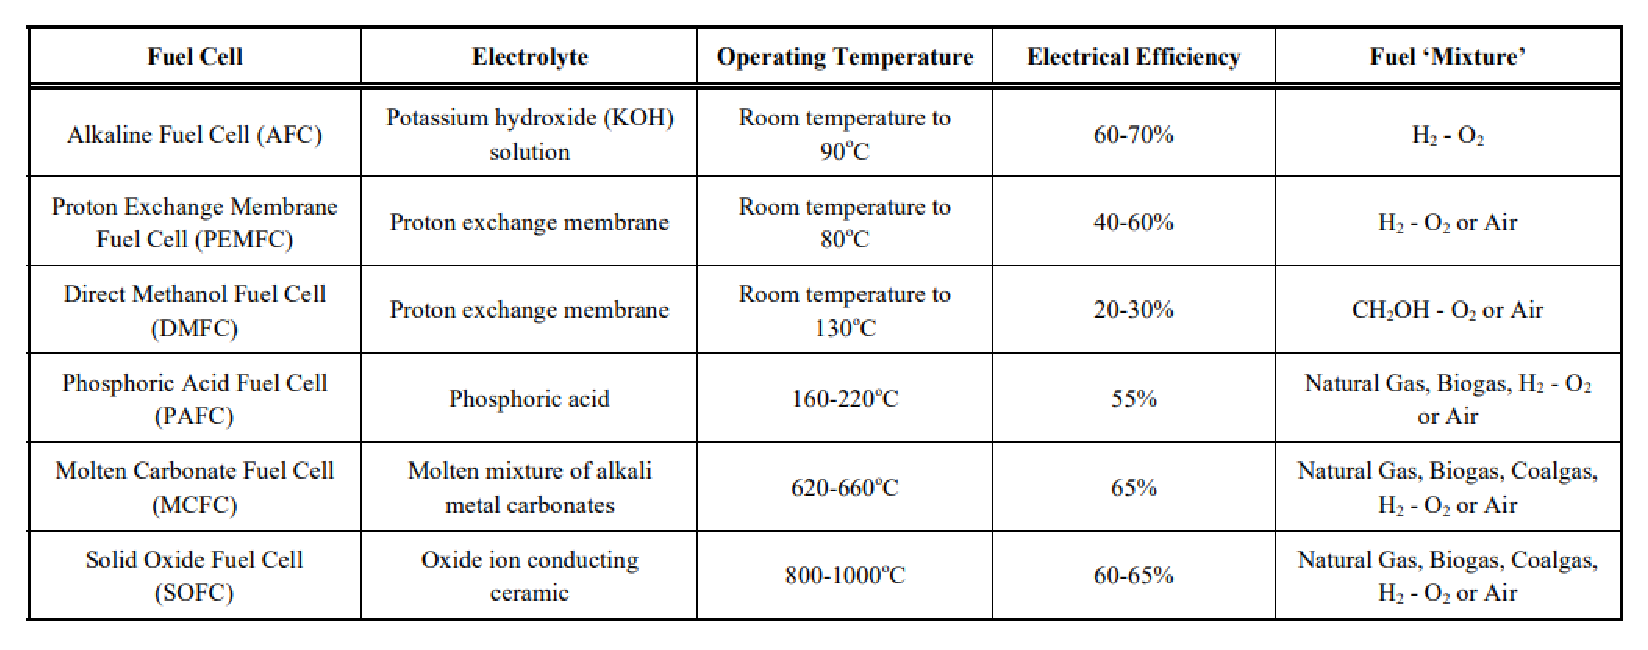
\includegraphics[scale=0.6]{images/fctypes}
\par\end{centering}
\caption{\label{fig:Different-fuel-cell}Different fuel cell types \citep{Panayiotou2010}}

\end{figure}

AFC are among the earliest researched fuel cell types and were mainly
used in space travel deployed. Operating efficiency: about 60\% to
70\%. Proton Exchange membrane fuel cells (PEMFC) use membrane foil
called Nafion and Electrodes with platinum layers as catalysts. They
are powered by hydrogen or finely purified reformate from simple hydrocarbons
such as natural gas, LPG or alcohols. These cells are used in home
power supplies, power plants, submarines and space travel and have
an efficiency of 40-60\%. Direct methanol fuel cells (DMFC) are operated
with liquid methanol and a membrane foil is used as the electrolyte.
Due to the low power density, these cells are mainly used as battery
chargers. Molten carbonate fuel cells (MCFC) have a molten carbonate
electrolyte. Because of the operating temperature of approx. 650�C
and the resulting high reaction speeds, therefore no expensive noble
metal catalysts are required. They are operated with desulfurized
natural and coal gas or suitably cleaned biogas. MCFC systems are
developed for the power plant range from 200 kW to several MW and
have an efficiency of 50\% to 65\%. Solid oxide fuel cells (SOFC)
are operated with a solid ceramic metal oxide as the electrolyte.
The operating temperature of 800�C enable that no expensive noble
metal catalysts are required. These cells can be operated with fossil
gases or biogas. SOFC systems are developed in the power range from
1 kW to 200 kW and have an efficiency of 60-65\% \citep{schaloske2012energietrager}.

\subsection{Challenges and solutions}

The fuel technology is mature in many areas and in regular operation.
In particular, passenger cars, forklifts and micro combined heat and
power plants (CHP) for residential buildings are among the mature
applications and are already commercially available, followed by buses,
emergency generators, industrial CHP plants and various network services.
However, there are many possible ones Hydrogen and fuel applications
Cells where no comparable experiences have been made so far and which
are still in the research and development phase. These include, for
example Trains, waste disposal vehicles and delivery vehicles, but
also heavy duty trucks as well airplanes and ships. The challenge
for the use of the technology also remains in terms of infrastructure
as well as expanding the filling stations for hydrogen. In addition
to the infrastructure The further development of the production facilities
is a challenge, especially in the transition to serial production.
For this reason Know-how transfer is essential for the market ramp-up,
to reduce existing reservations and gaps in knowledge \citep{weichenhain2020potenziale}.

\section{Electromagnetic reverberations chambers}

\bibliographystyle{unsrtdin}
\bibliography{bibtex-daten/bachelorarbeit-info}

\end{document}
